\section{Leave one out procedure for the clinical properties}
\label{sec:supp_studies}

The results section of the main paper reports the contribution of each clinical property. The procedure is
a leave one out ablation. At test time, one property at a time is switched off by setting its score
to the satisfied value and its failure map to zero, and the whole test set is re evaluated with that
property held-out. This is the same kind of one at a time removal used for the rule constants and for
the components of the method, applied here to the six clinical properties instead.

\section{Full per cell spreads}
\label{sec:supp_full_spreads}

The results table of the main paper prints each clinical cell as a mean, with the robustness
test folded into the choice of bold, and drops the per seed spread to keep the table one page.
Table~\ref{tab:supp_full_spreads} here restores that spread for every cell, four backbones by three
blocks by six measures, each as mean plus or minus one standard deviation across three seeds,
generated directly from the same result files.

\begin{table*}[!tb]
\centering
\caption{Every clinical cell of Tables 4 and 5 of the main paper, with its full mean plus or minus one seed
standard deviation restored. Each cell here is the one those tables show as a mean alone, and bold marks a mean that exceeds
its spread.}
\label{tab:supp_full_spreads}
\setlength{\tabcolsep}{4pt}
\footnotesize
\begin{tabular}{lcccccc}
\toprule
Backbone & $\Delta$CNR & $\Delta$TCI & $\Delta$EPI & $\Delta$BS & $\Delta$ENL & $\Delta$SNR \\
\midrule
\multicolumn{7}{l}{\textit{PKU37 test set, 173 images}} \\
\midrule
NAFNet & +3.49 $\pm$ 0.19 & +1.91 $\pm$ 0.51 & +1.20 $\pm$ 0.02 & +3.89 $\pm$ 0.45 & +23.74 $\pm$ 0.38 & +11.10 $\pm$ 0.31 \\
DnCNN & +11.30 $\pm$ 0.52 & +0.99 $\pm$ 1.62 & +4.14 $\pm$ 0.16 & -1.44 $\pm$ 0.87 & +57.14 $\pm$ 7.63 & +22.95 $\pm$ 2.28 \\
SwinIR & +7.33 $\pm$ 0.81 & +11.45 $\pm$ 0.86 & +2.68 $\pm$ 0.16 & +1.82 $\pm$ 0.37 & +28.32 $\pm$ 1.30 & +11.54 $\pm$ 0.26 \\
KBNet & +6.93 $\pm$ 0.98 & +5.92 $\pm$ 1.81 & +0.00 $\pm$ 0.07 & +2.58 $\pm$ 1.35 & +25.30 $\pm$ 2.17 & +7.95 $\pm$ 0.36 \\
\midrule
\multicolumn{7}{l}{\textit{Duke17, no adaptation}} \\
\midrule
NAFNet & +7.51 $\pm$ 0.21 & +4.00 $\pm$ 1.08 & +1.37 $\pm$ 0.07 & +4.15 $\pm$ 0.16 & +21.35 $\pm$ 1.78 & +5.43 $\pm$ 0.80 \\
DnCNN & +12.19 $\pm$ 0.72 & -1.47 $\pm$ 3.15 & +3.49 $\pm$ 0.15 & -2.24 $\pm$ 1.55 & +39.42 $\pm$ 5.44 & +13.55 $\pm$ 1.35 \\
SwinIR & +8.68 $\pm$ 1.12 & +13.26 $\pm$ 0.91 & +2.69 $\pm$ 0.24 & +1.90 $\pm$ 1.00 & +29.46 $\pm$ 0.66 & +11.60 $\pm$ 0.29 \\
KBNet & +5.34 $\pm$ 0.87 & +7.19 $\pm$ 1.57 & -0.50 $\pm$ 0.19 & +1.61 $\pm$ 0.09 & +7.49 $\pm$ 3.76 & -1.81 $\pm$ 1.80 \\
\midrule
\multicolumn{7}{l}{\textit{Duke2013, no adaptation}} \\
\midrule
NAFNet & +7.37 $\pm$ 0.06 & +1.41 $\pm$ 0.87 & +0.85 $\pm$ 0.04 & +0.51 $\pm$ 0.16 & +28.80 $\pm$ 2.25 & +9.29 $\pm$ 1.25 \\
DnCNN & +12.73 $\pm$ 1.41 & -2.21 $\pm$ 2.71 & +2.99 $\pm$ 0.25 & -5.85 $\pm$ 0.87 & +49.91 $\pm$ 7.29 & +17.59 $\pm$ 2.04 \\
SwinIR & +9.26 $\pm$ 1.20 & +11.86 $\pm$ 1.10 & +2.55 $\pm$ 0.20 & +2.30 $\pm$ 1.69 & +30.90 $\pm$ 1.02 & +13.31 $\pm$ 0.20 \\
KBNet & +7.16 $\pm$ 0.94 & +4.83 $\pm$ 1.32 & -0.35 $\pm$ 0.09 & +3.06 $\pm$ 1.03 & +8.70 $\pm$ 4.55 & -0.90 $\pm$ 2.14 \\
\bottomrule
\end{tabular}

\end{table*}

\section{The cooperation map, in full}
\label{sec:supp_cooperation}

The main paper reports that the map produced by the head reading the backbone features does not
predict the error of that backbone. This section gives the rest of the analysis.

Two measures were computed over the \NImages{} test images. The quantity correlated with the
absolute error of the backbone output is the demand map $\mathbf{u} = \mathbf{1} - \mathbf{c}$, which
is high where the wrapper is told to act. A demand map that tracked backbone error would give a
positive correlation. The measured rank correlation is \CalibRho{}, so the ordering runs the other
way. The sparsification error, the area between the curve obtained by removing the pixels the map
calls least reliable and the curve obtained by removing the pixels that are actually worst, is
\CalibAuse{}. A perfect ordering scores zero on the second measure and one on the first.

The reason is structural rather than a matter of tuning. The head is trained only through the
cooperation term of the objective, which rewards agreement between the map and the estimated
correction potential. That potential is itself a learned quantity. A map supervised only against
another learned map has no path by which the error of the backbone could reach it, so there is no
reason for it to acquire the meaning the original name implied.

Repairing this would require a term that regresses the map on the measured backbone error. Such a
term would compete with the cooperation term rather than complement it, because one pulls the map
toward the error of the backbone and the other pulls it toward where the correctors want to act. The
relative weight of the two would have to be selected, and every result in this paper would have to be
recomputed. We therefore report the measurement and leave the repair as the clearest piece of future
work this revision has identified.

\begin{figure*}[!tb]
\centering
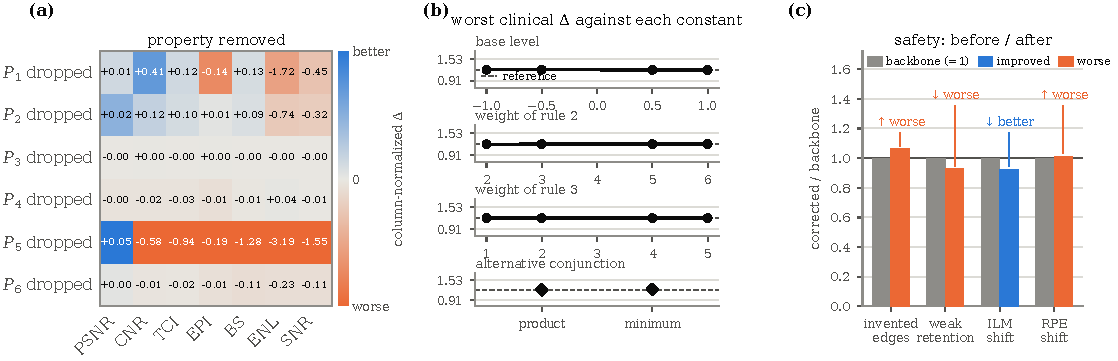
\includegraphics[width=0.86\textwidth]{figures/fig_studies.pdf}
\caption{The three studies of the main paper drawn together. Left, removing one clinical property at
a time, in points of the measure. Only $P_5$, $P_1$ and $P_2$ move any measure by more than a quarter
point, so $P_3$, $P_4$ and $P_6$ are close to inert here. Middle, the fourteen variations of the rule
constants, none of which turns a clinical measure negative, with the base allocation level the only
visible effect. Right, the safety analysis, each of the invented edge rate, weak structure retention
and the two boundary shifts shown as the ratio of corrected to backbone value, one meaning unchanged,
the arrow giving the direction and the word whether it is better or worse for that measure. Three
ratios sit on the worse side, though the retinal pigment epithelium shift moves one percent and is
not significant. All panels are the selected NAFNet checkpoint on the same \NImages{} test images.}
\label{fig:supp_studies}
\end{figure*}
